\documentclass[tikz,border=0.1cm]{standalone}
\usetikzlibrary{decorations.pathreplacing,positioning, arrows.meta}
\definecolor{Orange}{HTML}{fa7303}
\definecolor{Blue}{HTML}{0e0441}

\begin{document}
\newcommand{\ImageWidth}{7cm}

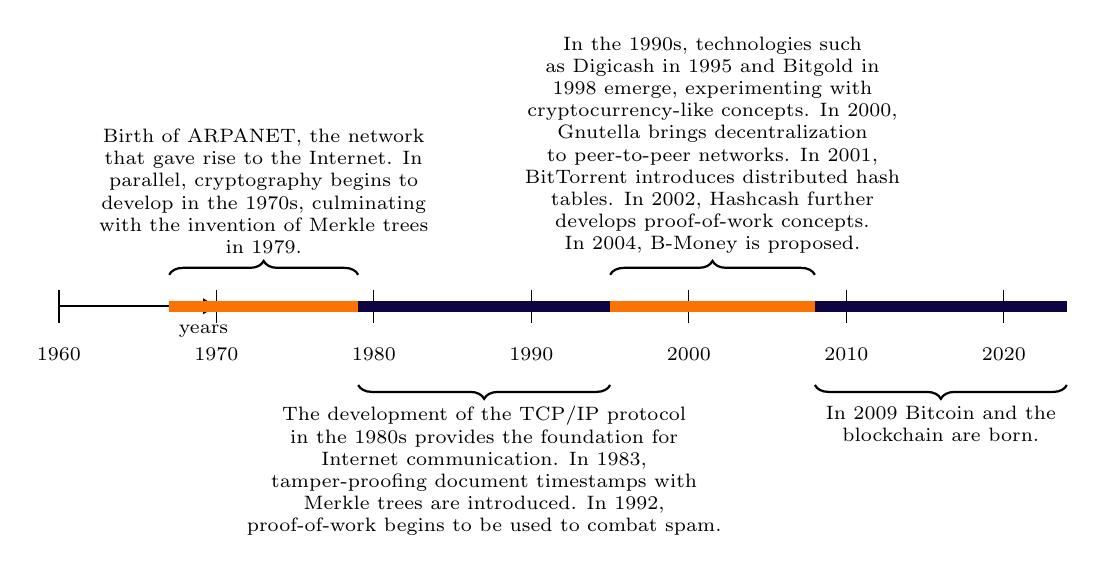
\begin{tikzpicture}[scale=2]
% draw horizontal line   
\draw[thick, -Triangle] (0,0) -- (\ImageWidth,0) node[font=\scriptsize,below left=3pt and -8pt]{years};

% draw vertical lines
\foreach \x in {0,1,...,6}
\draw (\x cm,3pt) -- (\x cm,-3pt);

\foreach \x/\descr in {0/1960,1/1970,2/1980,3/1990,4/2000,5/2010,6/2020}
\node[font=\scriptsize, text height=1.75ex,
text depth=.5ex] at (\x,-.3) {$\descr$};

% colored bar 
\foreach \x/\perccol in
{0.7/0,0.9/0}
\draw[lightgray!\perccol!Orange, line width=4pt] 
(\x,.0) -- +(1,0);

\foreach \x/\perccol in
{1.9/0,2.5/0}
\draw[lightgray!\perccol!Blue, line width=4pt] 
(\x,.0) -- +(1,0);

\foreach \x/\perccol in
{3.5/0, 3.8/0}
\draw[lightgray!\perccol!Orange, line width=4pt] 
(\x,.0) -- +(1,0);

\foreach \x/\perccol in
{4.8/0, 5.4/0}
\draw[lightgray!\perccol!Blue, line width=4pt] 
(\x,.0) -- +(1,0);

% braces
\draw [thick ,decorate,decoration={brace,amplitude=5pt}] (0.7,0.2)  -- +(1.2,0) 
       node [black,midway,above=4pt, font=\scriptsize, align=center] {Birth of ARPANET, the network \\ that gave rise to the Internet. In \\ parallel, cryptography begins to \\ develop in the 1970s, culminating \\ with the invention of Merkle trees \\ in 1979.};
\draw [thick,decorate,decoration={brace,amplitude=5pt}] (3.5,-.5) -- +(-1.6,0)
       node [black,midway,font=\scriptsize, below=4pt, align=center] {The development of the TCP/IP protocol \\ in the 1980s provides the foundation for \\ Internet communication. In 1983, \\ tamper-proofing document timestamps with \\ Merkle trees are introduced. In 1992, \\ proof-of-work begins to be used to combat spam.};
\draw [thick ,decorate,decoration={brace,amplitude=5pt}] (3.5,0.2)  -- +(1.3,0) 
       node [black,midway, above=4pt, font=\scriptsize, align=center] {In the 1990s, technologies such \\ as Digicash in 1995 and Bitgold in \\ 1998 emerge, experimenting with \\ cryptocurrency-like concepts. In 2000, \\ Gnutella brings decentralization \\to peer-to-peer networks. In 2001, \\ BitTorrent introduces distributed hash \\ tables. In 2002, Hashcash further \\ develops proof-of-work concepts. \\ In 2004, B-Money is proposed.};
\draw [thick,decorate,decoration={brace,amplitude=5pt}] (6.4,-.5) -- +(-1.6,0)
       node [black,midway,font=\scriptsize, below=4pt, align=center] {In 2009 Bitcoin and the \\ blockchain are born.};
\end{tikzpicture}

\end{document}

